\documentclass[border=5pt]{standalone}
\usepackage{tikz}
\usepackage{amsmath}
\begin{document}
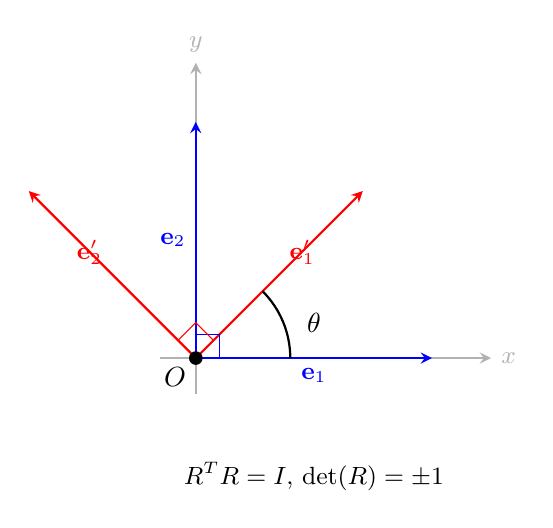
\begin{tikzpicture}[scale=1.5, >=stealth]
  % Orthogonal matrix: rotation preserves lengths and angles

  % Original axes
  \draw[->, thick, gray!60] (-0.3,0) -- (2.5,0) node[right, font=\small] {$x$};
  \draw[->, thick, gray!60] (0,-0.3) -- (0,2.5) node[above, font=\small] {$y$};

  % Original vectors
  \draw[->, thick, blue] (0,0) -- (2,0) node[midway, below, font=\small] {$\mathbf{e}_1$};
  \draw[->, thick, blue] (0,0) -- (0,2) node[midway, left, font=\small] {$\mathbf{e}_2$};

  % Rotated vectors
  \draw[->, thick, red] (0,0) -- (1.414, 1.414) node[midway, above right, font=\small] {$\mathbf{e}_1'$};
  \draw[->, thick, red] (0,0) -- (-1.414, 1.414) node[midway, above left, font=\small] {$\mathbf{e}_2'$};

  % Rotation angle
  \draw[thick] (0.8, 0) arc (0:45:0.8);
  \node at (1, 0.3) {$\theta$};

  % Right angles
  \draw[blue, thin] (0.2, 0) -- (0.2, 0.2) -- (0, 0.2);
  \draw[red, thin] (0.15, 0.15) -- (0, 0.3) -- (-0.15, 0.15);

  % Origin
  \filldraw[black] (0,0) circle (1.5pt) node[below left] {$O$};

  % Formula
  \node[font=\small] at (1, -1) {$R^T R = I$, $\det(R) = \pm 1$};
\end{tikzpicture}
\end{document}
